\chapter{Результаты} \label{chapt3}


\section{Незвешенные графы} \label{sect3_1}

Результаты экспериментов представлены на графиках.
Во всех случаях по оси $x$ отложены значения параметра семейства. Для удобства все параметры были отнормированы на отрезок $[0,1]$ с помощью дробно-линейного преобразования.

\begin{figure}[h]
  \begin{minipage}[h]{0.49\linewidth}
    \center{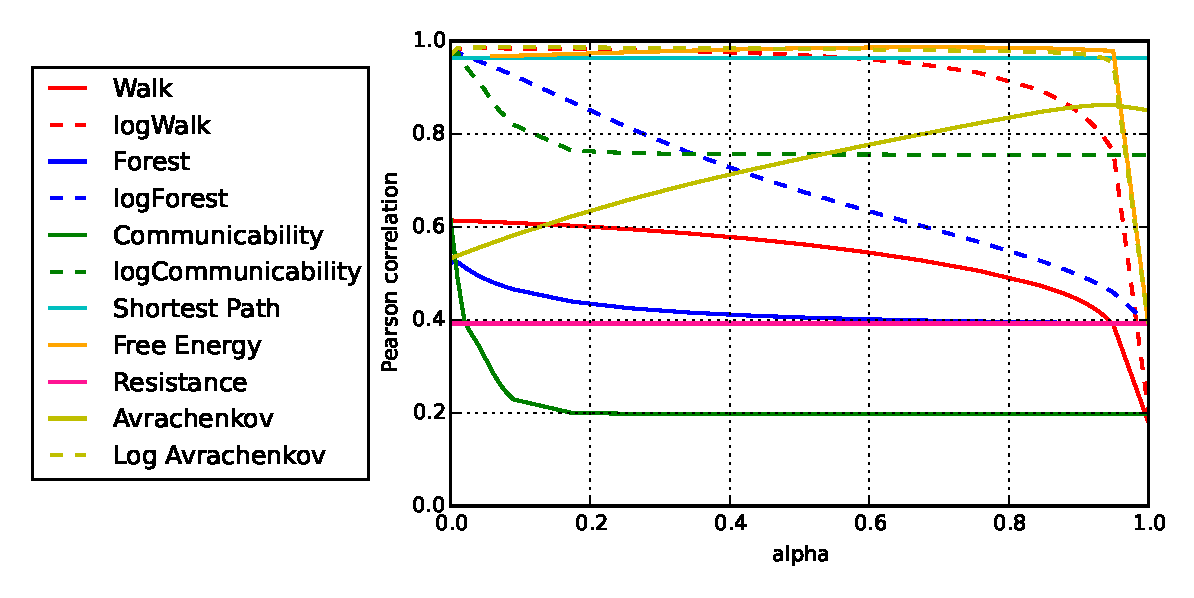
\includegraphics[width=0.95\linewidth]{correlations_eps} \\ а)}
  \end{minipage}
  \hfill
  \begin{minipage}[h]{0.49\linewidth}
    \center{\includegraphics[width=0.95\linewidth]{correlations_zoom_eps} \\ б)}
  \end{minipage}

  \caption{Корреляции для $\varepsilon$-графов}
  \label{img:eps_graphs}  
\end{figure}

%===========================================
\begin{table} [htbp]
  \centering
  \parbox{15cm}{\caption{Параметры метрик для $\varepsilon$ - графов}\label{Ts0Sib}}
%  \begin{center}
  \begin{tabular}{| p{6cm} || p{2cm} | p{2cm} | p{2cm}l |}
  \hline
  \hline
  Метрика   & \centering Значение параметра из $[0,1]$ & \centering Наилучшая степень &\centering  Корреляция & \\
  \hline
  Walk &\centering  1.0   &\centering  1.0    &\centering      4.203  &   \\
  \hline
  Log Walk  &\centering  262.431   &\centering  1.0    &\centering      0.783  &   \\
  \hline
  Forest &\centering  261.184   &\centering  260.381    &\centering     $-$0.803  &   \\
  \hline
  Log Forest &\centering  253.575   &\centering  257.778    &\centering      4.203  &   \\
  \hline
  Communicability &\centering  253.575   &\centering  257.778    &\centering      4.203  &   \\
  \hline
  Log Communicability &\centering  253.575   &\centering  257.778    &\centering      4.203  &   \\
  \hline
  Shortest Path &\centering  не зависит   &\centering  257.778    &\centering      4.203  &   \\
  \hline
  Resistance &\centering  не зависит   &\centering  257.778    &\centering      4.203  &   \\
  \hline
  Free Energy &\centering  253.575   &\centering  257.778    &\centering      4.203  &   \\
  \hline
  Avrachenkov, $\sigma = 0$ &\centering  253.575   &\centering  257.778    &\centering      4.203  &   \\
  \hline
  Avrachenkov, $\sigma = 0.25$ &\centering  253.575   &\centering  257.778    &\centering      4.203  &   \\
  \hline
  Avrachenkov, $\sigma = 0.5$ &\centering  253.575   &\centering  257.778    &\centering      4.203  &   \\
  \hline
  Avrachenkov, $\sigma = 0.75$ &\centering  253.575   &\centering  257.778    &\centering      4.203  &   \\
  \hline
  Avrachenkov, $\sigma = 1$ &\centering  253.575   &\centering  257.778    &\centering      4.203  &   \\
  \hline
  Log Avrachenkov, $\sigma = 0$ &\centering  253.575   &\centering  257.778    &\centering      4.203  &   \\
  \hline
  Log Avrachenkov, $\sigma = 0.25$ &\centering  253.575   &\centering  257.778    &\centering      4.203  &   \\
  \hline
  Log Avrachenkov, $\sigma = 0.5$ &\centering  253.575   &\centering  257.778    &\centering      4.203  &   \\
  \hline
  Log Avrachenkov, $\sigma = 0.75$ &\centering  253.575   &\centering  257.778    &\centering      4.203  &   \\
  \hline
  Log Avrachenkov, $\sigma = 1$ &\centering  253.575   &\centering  257.778    &\centering      4.203  &   \\
  \hline
  \hline
  \end{tabular}
%  \end{center}
\end{table}

%===========================================

\begin{figure}[h]
  \begin{minipage}[h]{0.49\linewidth}
    \center{\includegraphics[width=0.95\linewidth]{correlations_sym} \\ а)}
  \end{minipage}
  \hfill
  \begin{minipage}[h]{0.49\linewidth}
    \center{\includegraphics[width=0.95\linewidth]{correlations_zoom_sym} \\ б)}
  \end{minipage}

  \caption{Корреляции для симметричных графов ближайших соседей}
  \label{img:sym_graphs}  
\end{figure}

%===========================================

Значения параметров, при которых метрики лучше всего приближают евклидово расстояние для каждого типа графов, приведены в таблице:


\begin{table} [htbp]
  \centering
  \parbox{15cm}{\caption{Параметры метрик для симметричных графов ближайших соседей}\label{Ts0Sib}}
%  \begin{center}
  \begin{tabular}{| p{6cm} || p{2cm} | p{2cm} | p{2cm}l |}
  \hline
  \hline
  Метрика   & \centering Значение параметра из $[0,1]$ & \centering Наилучшая степень &\centering  Корреляция & \\
  \hline
  Walk &\centering  1.0   &\centering  1.0    &\centering      4.203  &   \\
  \hline
  Log Walk  &\centering  262.431   &\centering  1.0    &\centering      0.783  &   \\
  \hline
  Forest &\centering  261.184   &\centering  260.381    &\centering     $-$0.803  &   \\
  \hline
  Log Forest &\centering  253.575   &\centering  257.778    &\centering      4.203  &   \\
  \hline
  Communicability &\centering  253.575   &\centering  257.778    &\centering      4.203  &   \\
  \hline
  Log Communicability &\centering  253.575   &\centering  257.778    &\centering      4.203  &   \\
  \hline
  Shortest Path &\centering  не зависит   &\centering  257.778    &\centering      4.203  &   \\
  \hline
  Resistance &\centering  не зависит   &\centering  257.778    &\centering      4.203  &   \\
  \hline
  Free Energy &\centering  253.575   &\centering  257.778    &\centering      4.203  &   \\
  \hline
  Avrachenkov, $\sigma = 0$ &\centering  253.575   &\centering  257.778    &\centering      4.203  &   \\
  \hline
  Avrachenkov, $\sigma = 0.25$ &\centering  253.575   &\centering  257.778    &\centering      4.203  &   \\
  \hline
  Avrachenkov, $\sigma = 0.5$ &\centering  253.575   &\centering  257.778    &\centering      4.203  &   \\
  \hline
  Avrachenkov, $\sigma = 0.75$ &\centering  253.575   &\centering  257.778    &\centering      4.203  &   \\
  \hline
  Avrachenkov, $\sigma = 1$ &\centering  253.575   &\centering  257.778    &\centering      4.203  &   \\
  \hline
  Log Avrachenkov, $\sigma = 0$ &\centering  253.575   &\centering  257.778    &\centering      4.203  &   \\
  \hline
  Log Avrachenkov, $\sigma = 0.25$ &\centering  253.575   &\centering  257.778    &\centering      4.203  &   \\
  \hline
  Log Avrachenkov, $\sigma = 0.5$ &\centering  253.575   &\centering  257.778    &\centering      4.203  &   \\
  \hline
  Log Avrachenkov, $\sigma = 0.75$ &\centering  253.575   &\centering  257.778    &\centering      4.203  &   \\
  \hline
  Log Avrachenkov, $\sigma = 1$ &\centering  253.575   &\centering  257.778    &\centering      4.203  &   \\
  \hline
  \hline
  \end{tabular}
%  \end{center}
\end{table}

%=================================


\begin{figure}[h]
  \begin{minipage}[h]{0.49\linewidth}
    \center{\includegraphics[width=0.95\linewidth]{correlations_mut} \\ а)}
  \end{minipage}
  \hfill
  \begin{minipage}[h]{0.49\linewidth}
    \center{\includegraphics[width=0.95\linewidth]{correlations_zoom_mut} \\ б)}
  \end{minipage}

  \caption{Корреляции для mutual графов ближайших соседей}
  \label{img:mut_graphs}  
\end{figure}

%===========================================

\begin{table} [htbp]
  \centering
  \parbox{15cm}{\caption{Параметры метрик для mutual графов ближайших соседей}\label{Ts0Sib}}
%  \begin{center}
  \begin{tabular}{| p{6cm} || p{2cm} | p{2cm} | p{2cm}l |}
  \hline
  \hline
  Метрика   & \centering Значение параметра из $[0,1]$ & \centering Наилучшая степень &\centering  Корреляция & \\
  \hline
  Walk &\centering  1.0   &\centering  1.0    &\centering      4.203  &   \\
  \hline
  Log Walk  &\centering  262.431   &\centering  1.0    &\centering      0.783  &   \\
  \hline
  Forest &\centering  261.184   &\centering  260.381    &\centering     $-$0.803  &   \\
  \hline
  Log Forest &\centering  253.575   &\centering  257.778    &\centering      4.203  &   \\
  \hline
  Communicability &\centering  253.575   &\centering  257.778    &\centering      4.203  &   \\
  \hline
  Log Communicability &\centering  253.575   &\centering  257.778    &\centering      4.203  &   \\
  \hline
  Shortest Path &\centering  не зависит   &\centering  257.778    &\centering      4.203  &   \\
  \hline
  Resistance &\centering  не зависит   &\centering  257.778    &\centering      4.203  &   \\
  \hline
  Free Energy &\centering  253.575   &\centering  257.778    &\centering      4.203  &   \\
  \hline
  Avrachenkov, $\sigma = 0$ &\centering  253.575   &\centering  257.778    &\centering      4.203  &   \\
  \hline
  Avrachenkov, $\sigma = 0.25$ &\centering  253.575   &\centering  257.778    &\centering      4.203  &   \\
  \hline
  Avrachenkov, $\sigma = 0.5$ &\centering  253.575   &\centering  257.778    &\centering      4.203  &   \\
  \hline
  Avrachenkov, $\sigma = 0.75$ &\centering  253.575   &\centering  257.778    &\centering      4.203  &   \\
  \hline
  Avrachenkov, $\sigma = 1$ &\centering  253.575   &\centering  257.778    &\centering      4.203  &   \\
  \hline
  Log Avrachenkov, $\sigma = 0$ &\centering  253.575   &\centering  257.778    &\centering      4.203  &   \\
  \hline
  Log Avrachenkov, $\sigma = 0.25$ &\centering  253.575   &\centering  257.778    &\centering      4.203  &   \\
  \hline
  Log Avrachenkov, $\sigma = 0.5$ &\centering  253.575   &\centering  257.778    &\centering      4.203  &   \\
  \hline
  Log Avrachenkov, $\sigma = 0.75$ &\centering  253.575   &\centering  257.778    &\centering      4.203  &   \\
  \hline
  Log Avrachenkov, $\sigma = 1$ &\centering  253.575   &\centering  257.778    &\centering      4.203  &   \\
  \hline
  \hline
  \end{tabular}
%  \end{center}
\end{table}

Можем видеть, что логарифмические метрики позволяют более точно восстановить евклидово расстояние, чем метрики без логарифма.

*ОПИСАТЬ, КАК СЕБЯ ВЕДУТ МЕТРИКИ ПРИ ИЗМЕНЕНИИ ПАРАМЕТРОВ ГРАФА:
с ростом сигмы во взвешенных быстро все спадает
с ростом к и эпсилон???
Что происходит, когда граф распадается на кластеры?*

*****


**про оптимальные степени**


%\newpage
%============================================================================================================================
\clearpage

\section{Взвешенные графы} \label{sect3_2}

На графиках представлены результаты сравнения метрик с евклидовым расстоянием для взвешенных Гауссовских графов.

******

Видно, что в данном случае расстояние кратчайшего пути позволяет восстановить евклидово расстояние с точностью до константы. Это связано с особенностями определения весов ребер.

Наилучшие значения параметров для остальных метрик приведены в таблице:

****



\clearpage